\documentclass[11pt]{article} 
\usepackage{mathtools}
\usepackage[letterpaper, width=14cm, height=22cm, top=5cm]{geometry}       
 \headsep=1pt
\usepackage[parfill]{parskip}    % Activate to begin paragraphs with an empty line rather than an indent
\usepackage{graphicx}
\graphicspath{{./Images/}}
\usepackage{amssymb}
\usepackage{epstopdf}
\usepackage[usenames,dvipsnames]{color}
\usepackage{hyperref}
\hypersetup{colorlinks, urlcolor=Cyan, citecolor=Cyan, hyperfootnotes=false}
\usepackage[none]{hyphenat}

\usepackage{cite}
\setlength{\voffset}{-2cm}
\addtolength{\textheight}{2cm}
\addtolength{\textwidth}{3cm}
\addtolength{\hoffset}{-1.5cm}
\usepackage{fancyhdr}
\hyphenchar\font=-1

\begin{document}
C. S. Gorham\\
 \today 

2) KMCS\_irreversible.py is a kinetic monte carlo simulation (KMCS) modeling the catalytic conversion of A to B, in extension to the co-adsorption of A, and sole desorption of B on a square lattice of finite size. A and B available in abundance. The following are situations for which the simulation is run. The results are depicted through the figures herein and are described briefly. Further, the applicable .csv files are indicated and attached. \\

{\bf{Figure 1 - Different Lattice sizes; All transition coefficients equal}}\\
\hspace*{1cm}It is clear from the results that restricting the number of sites that contribute to the event probability below a certain size leads to size effects characterized by increased noise, i.e., increased signal fluctuation from equilibrium results, and greater apparent time between events which is an artifact of the simulation. Thus, when conducting a KMCS it is important to ensure that the experimental system is large enough to avoid size effects. 


{\bf{ Figure 2 - Smaller transition coefficients; All transition coefficients equal }} \\
\hspace*{1cm}When the transition coefficients are relatively small, events are able to occur more often as less energy is required for the event. Thus, there is shorter time between events and equilibrium is reached after a shorter amount of time. The system also exhibits a smaller temperature dependence due to the fact that the activation energy in the numerator of the exponential factor dominates the exponent.


{\bf{Figure 3 - Larger transition coefficients; All transition coefficients equal}}\\
\hspace*{1cm}When the transition coefficients are relatively large, less events are able to occur because a greater amount of energy is required for the event to occur. Thus, there is longer time between events and equilibrium is reached after a longer amount of time. The system also exhibits a much larger temperature dependence due to the fact that the activation energy in the numerator of the exponential factor dominates the exponent.


{\bf{Figure 4 - A-absorb activation energy 2x}}\\
When the activation energy for absorption events of a single family of particles is twice as large as that for all other events, all other events are much more likely to occur while these particles are unlikely to absorb. Thus, the total coverage of the system is very low because it is more likely that any absorbed particle will transition to B and/or desorb before another particle is absorbed. 

{\bf{Figure 5 - A-desorb activation energy 2x}}\\
When the activation energy for desorption events of a single family of particles is twice as large as that for all other events, all other events are much more likely to occur while these particles are unlikely to desorb. Thus, the total coverage of the system is very high because it is more likely that any particles will continue to absorb rather than desorb. 


{\bf{Figure 6 - B-desorb activation energy 2x}}\\
When the activation energy for desorption events of a single family of particles which is only created through a catalytic conversion is twice as large as that for all other events, all other events are much more likely to occur while these particles are unlikely to desorb. Thus, the total coverage of this family of particles on the system is very high because it is more likely that any particles will continue to absorb and transition to this family rather than particles from this family desorbing.


{\bf{Figure 7 - All-desorb activation energy 2x}}\\
When the activation energy for desorption events is twice as large as that for all other events, all other events are much more likely to occur while these particles are unlikely to desorb. Thus, in this simulation, the absorption of B and the transition of A to B are more likely to happen, which results in a high total coverage of the system.


{\bf{Figure 8 - A-B activation energy 2x}}\\
When the activation energy for catalytic transition of A to B is twice as large as that for all other events, all other events are much more likely to occur. Thus, very few B particles participate in this simulation - nearly none at lower temperatures.













\begin{figure}[h!]
\begin{tabular}{cc}
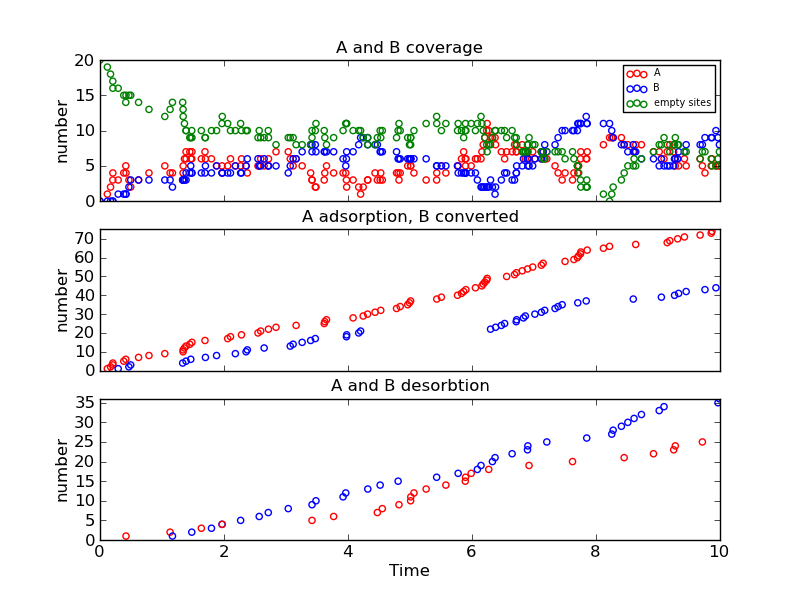
\includegraphics[width=3.5in, height=4.2in]{./coadsorb_irreversible/AtoBirreversible2x10_301_allsamek_A5_EA5E3_3.png} &
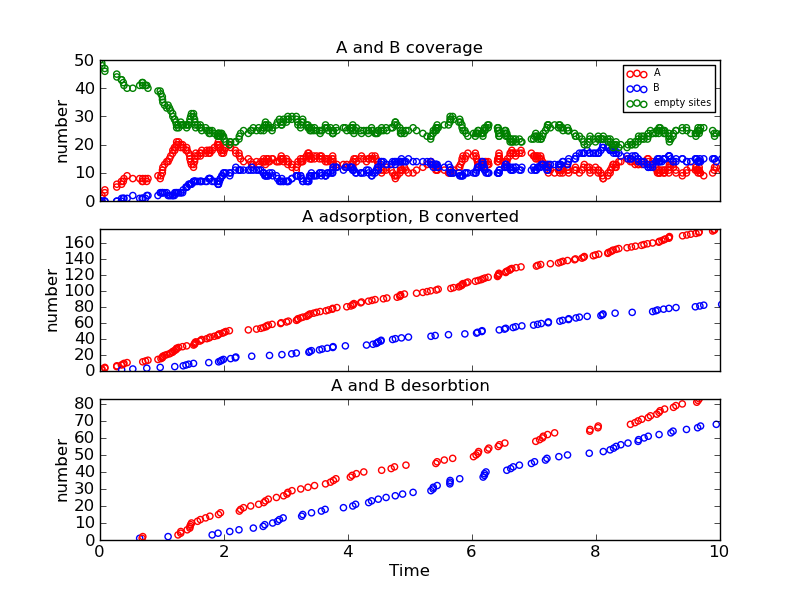
\includegraphics[width=3.5in, height=4.2in]{./coadsorb_irreversible/AtoBirreversible5x10_301_allsamek_A5_EA5E3_3.png} \\
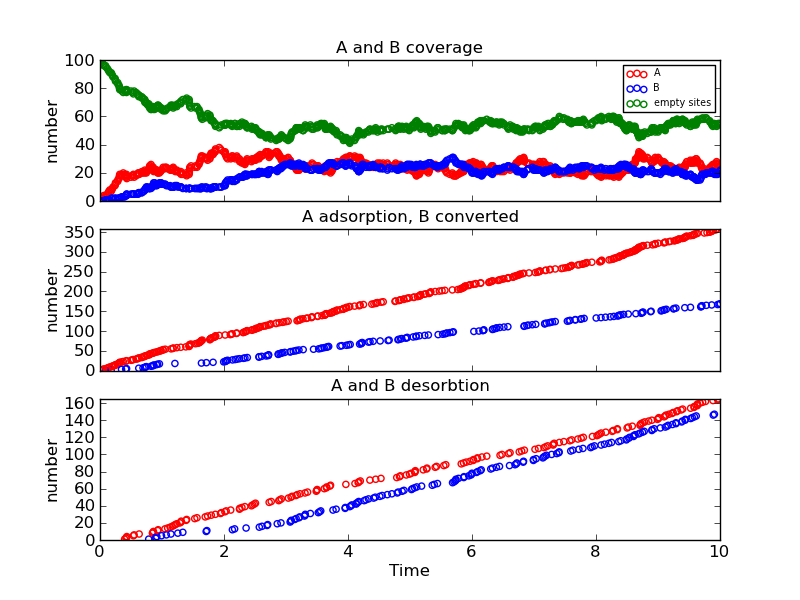
\includegraphics[width=3.5in, height=4.2in]{./coadsorb_irreversible/AtoBirreversible10x10_301_allsamek_A5_EA5E3_3.png} &
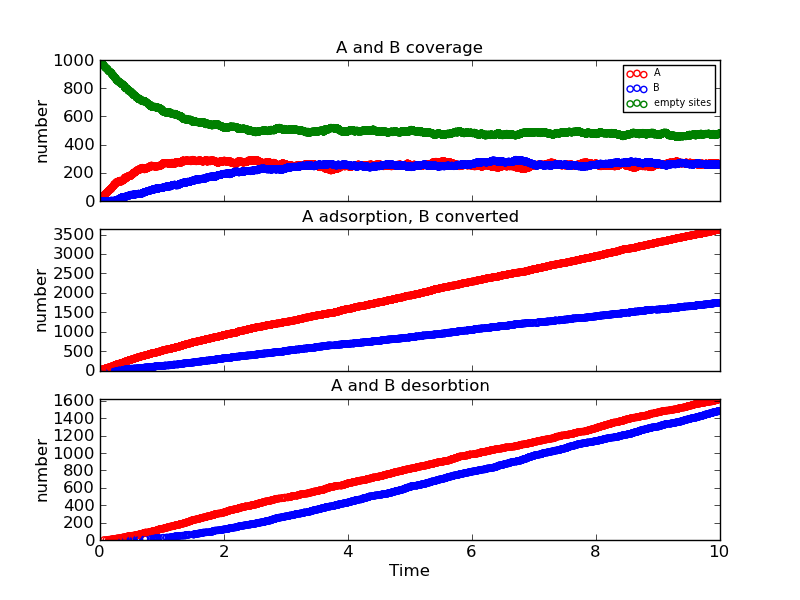
\includegraphics[width=3.5in, height=4.2in]{./coadsorb_irreversible/AtoBirreversible100x10_301_allsamek_A5_EA5E3_3.png} 
\end{tabular}
\caption{The figures depict the effect (top of three:) total coverage of the systems simulated, (middle of three:) absorption of the particles present, (bottom of three:) and desorption of the particles present using different lattice sizes in the KMCS, where the transition coefficients do not depend on the position of the lattice. All simulations are run at 301K. In these simulations, all events have the same transition coefficient, where the activation energy is E$_a$=5kJmol$^{-1}$. [From top left to bottom right:] 2x10, 5x10, 10x10, 100x10. }
\end{figure}

\setlength{\unitlength}{1in}
\begin{figure}[h!]
\begin{tabular}{cc}
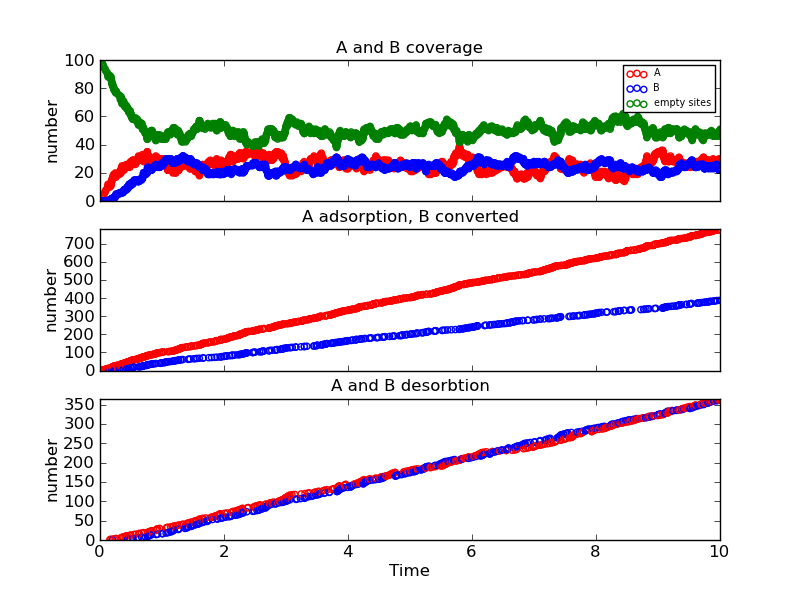
\includegraphics[width=3.5in, height=4.2in]{./coadsorb_irreversible/AtoBirreversible10x10_101_allsameksmall_A5_EA1E3_3.png} &
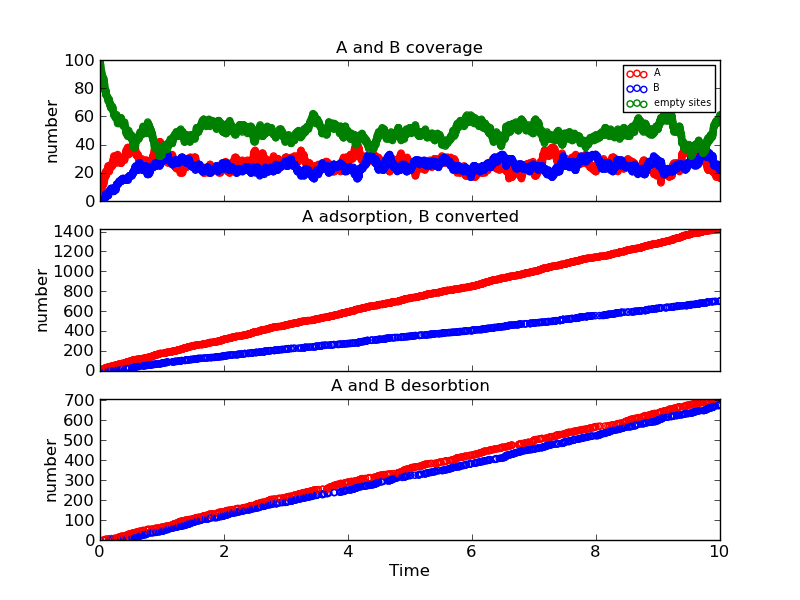
\includegraphics[width=3.5in, height=4.2in]{./coadsorb_irreversible/AtoBirreversible10x10_201_allsameksmall_A5_EA1E3_3.png} \\
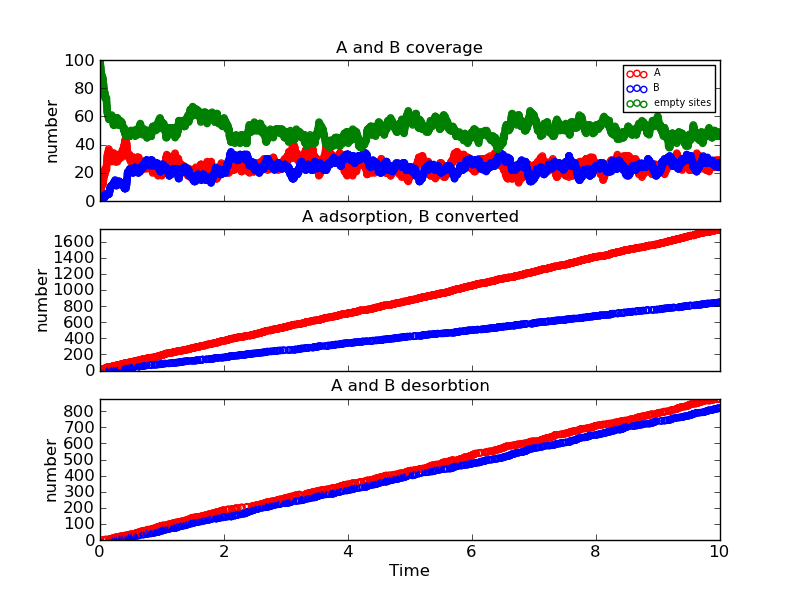
\includegraphics[width=3.5in, height=4.2in]{./coadsorb_irreversible/AtoBirreversible10x10_301_allsameksmall_A5_EA1E3_3.png} &
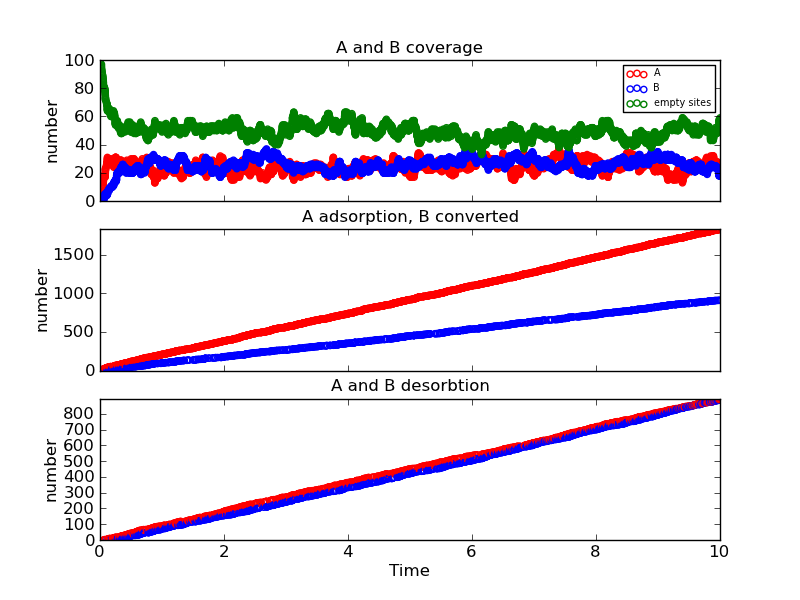
\includegraphics[width=3.5in, height=4.2in]{./coadsorb_irreversible/AtoBirreversible10x10_401_allsameksmall_A5_EA1E3_3.png} 
\end{tabular}
\caption{This figure describes the (top of three:) total coverage of the systems simulated, (middle of three:) absorption of the particles present, (bottom of three:) and desorption of the particles present on a 10x10 lattice, where the transition coefficients to not depend on the position of the lattice. In these simulations, all events have the same transition coefficient, where the activation energy is E$_a$=1kJmol$^{-1}$. [From top left to bottom right:] 101 K, 201 K, 301 K, 401 K. }
\end{figure}

\setlength{\unitlength}{1in}
\begin{figure}[h!]
\begin{tabular}{cc}
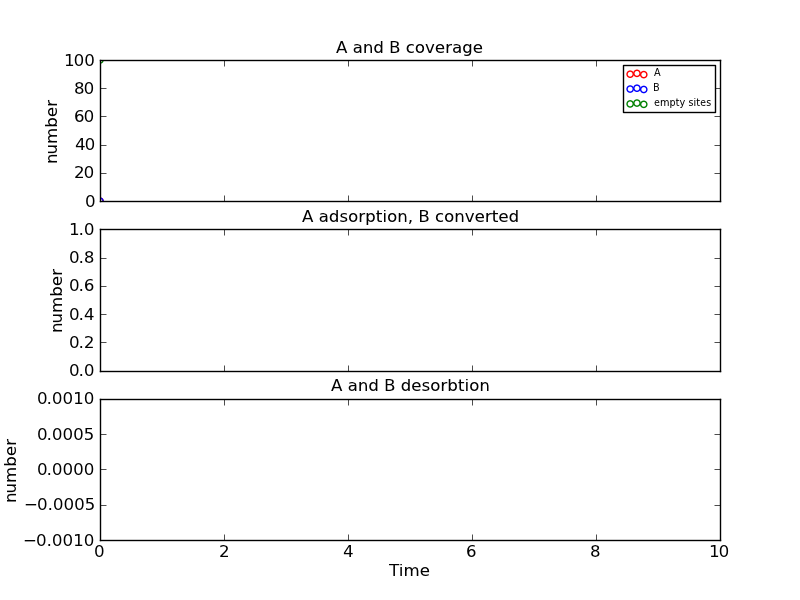
\includegraphics[width=3.5in, height=4.2in]{./coadsorb_irreversible/AtoBirreversible10x10_101_allsameklarge_A5_EA10E3_3.png} &
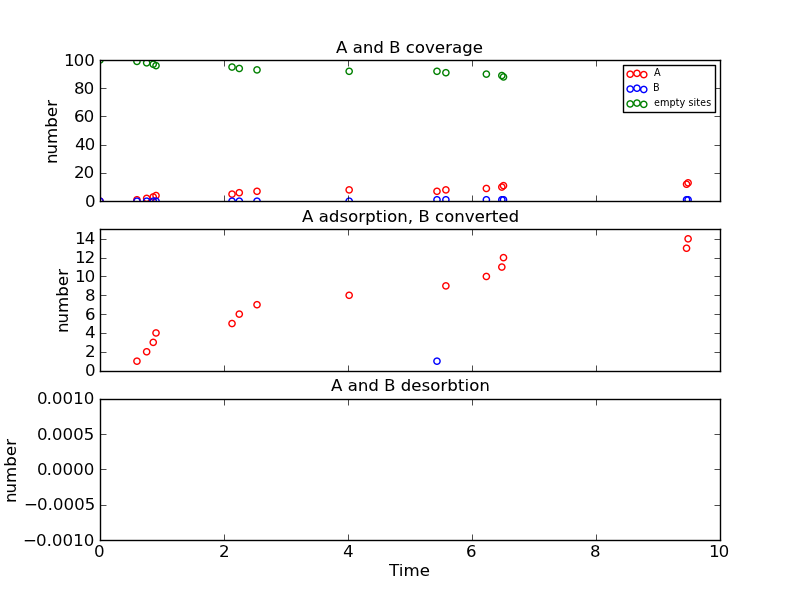
\includegraphics[width=3.5in, height=4.2in]{./coadsorb_irreversible/AtoBirreversible10x10_201_allsameklarge_A5_EA10E3_3.png} \\
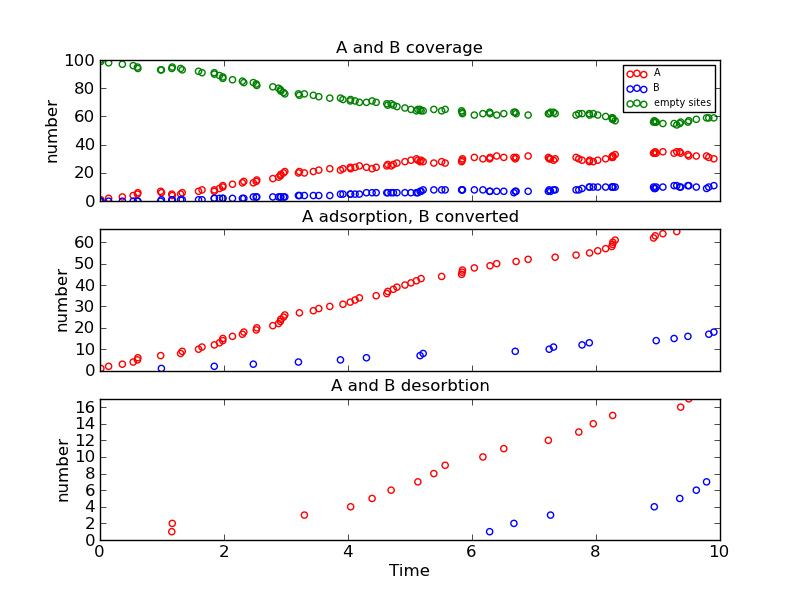
\includegraphics[width=3.5in, height=4.2in]{./coadsorb_irreversible/AtoBirreversible10x10_301_allsameklarge_A5_EA10E3_3.png} &
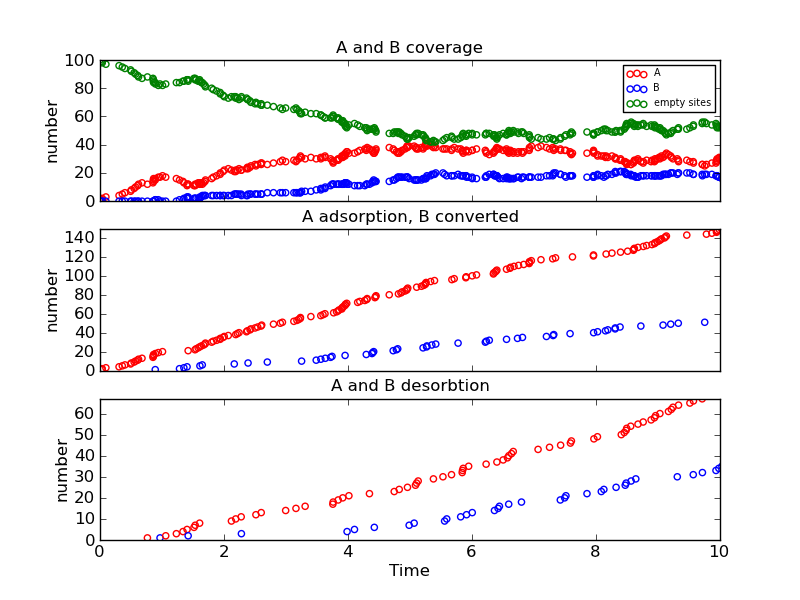
\includegraphics[width=3.5in, height=4.2in]{./coadsorb_irreversible/AtoBirreversible10x10_401_allsameklarge_A5_EA10E3_3.png} 
\end{tabular}
\caption{This figure describes the (top of three:) total coverage of the systems simulated, (middle of three:) absorption of the particles present, (bottom of three:) and desorption of the particles present on a 10x10 lattice, where the activation energy does not depend on the position of the lattice. In these simulations, all events have the same transition coefficient, where the activation energy is E$_a$=10kJmol$^{-1}$. [From top left to bottom right:] 101 K, 201 K, 301 K, 401 K.}
\end{figure}

\setlength{\unitlength}{1in}
\begin{figure}[h!]
\begin{tabular}{cc}
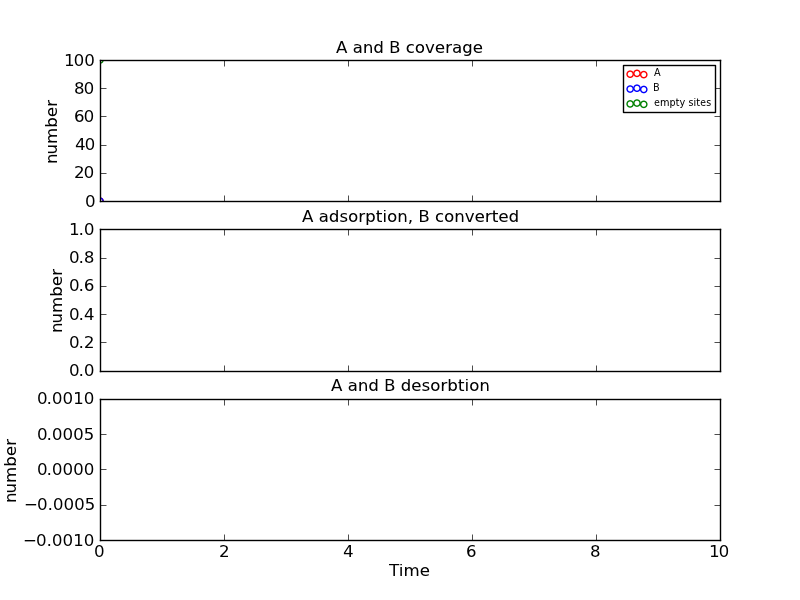
\includegraphics[width=3.5in, height=4.2in]{./coadsorb_irreversible/AtoBirreversible10x10_101_Aabs2x_EA10E3_EB5E3_3.png} &
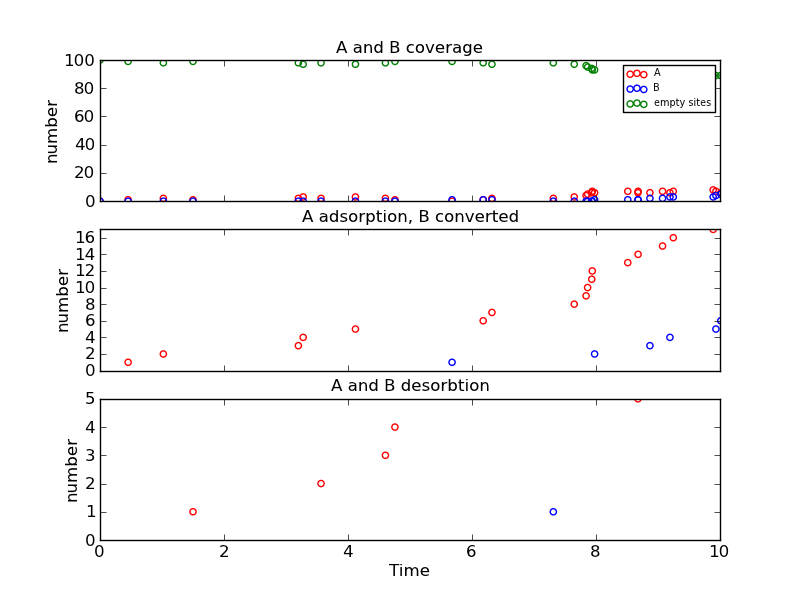
\includegraphics[width=3.5in, height=4.2in]{./coadsorb_irreversible/AtoBirreversible10x10_201_Aabs2x_EA10E3_EB5E3_3.png} \\
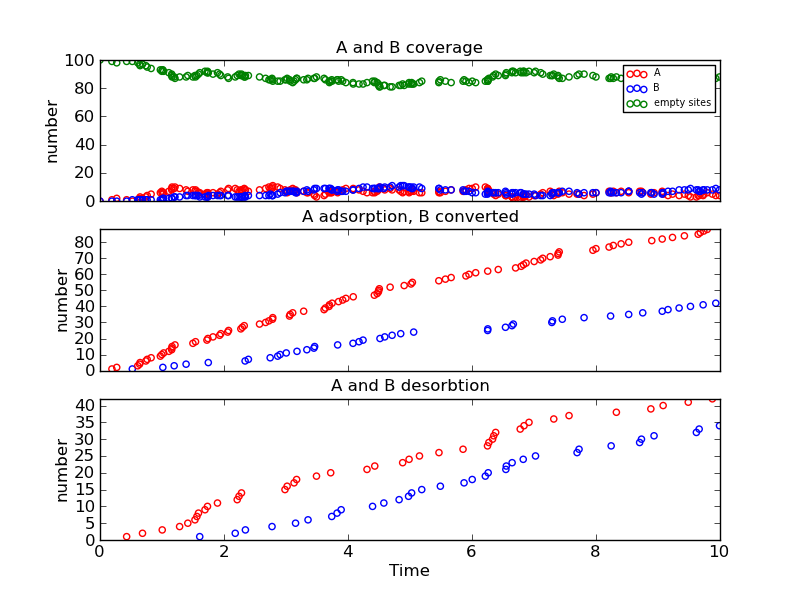
\includegraphics[width=3.5in, height=4.2in]{./coadsorb_irreversible/AtoBirreversible10x10_301_Aabs2x_EA10E3_EB5E3_3.png} &
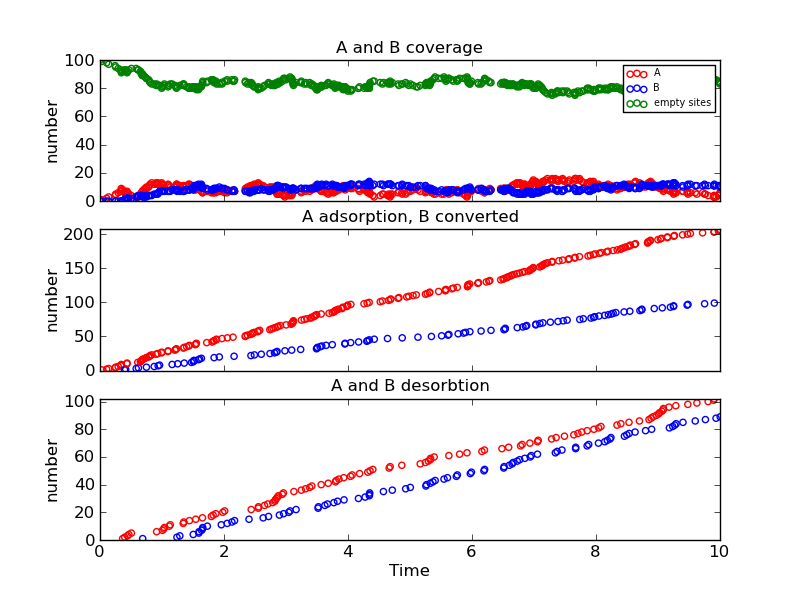
\includegraphics[width=3.5in, height=4.2in]{./coadsorb_irreversible/AtoBirreversible10x10_401_Aabs2x_EA10E3_EB5E3_3.png} 
\end{tabular}
\caption{This figure describes the (top of three:) total coverage of the systems simulated, (middle of three:) absorption of the particles present, (bottom of three:) and desorption of the particles present on a 10x10 lattice, where the transition coefficients to not depend on the position of the lattice. In these simulations, the activation energy of absorption of A is twice as large as any other event , where the activation energy is E$_{a_{A:absorption}}$=10kJmol$^{-1}$ and E$_{a_{other}}$=5kJmol$^{-1}$. [From top left to bottom right:] 101 K, 201 K, 301 K, 401 K. }
\end{figure}

\setlength{\unitlength}{1in}
\begin{figure}[h!]
\begin{tabular}{cc}
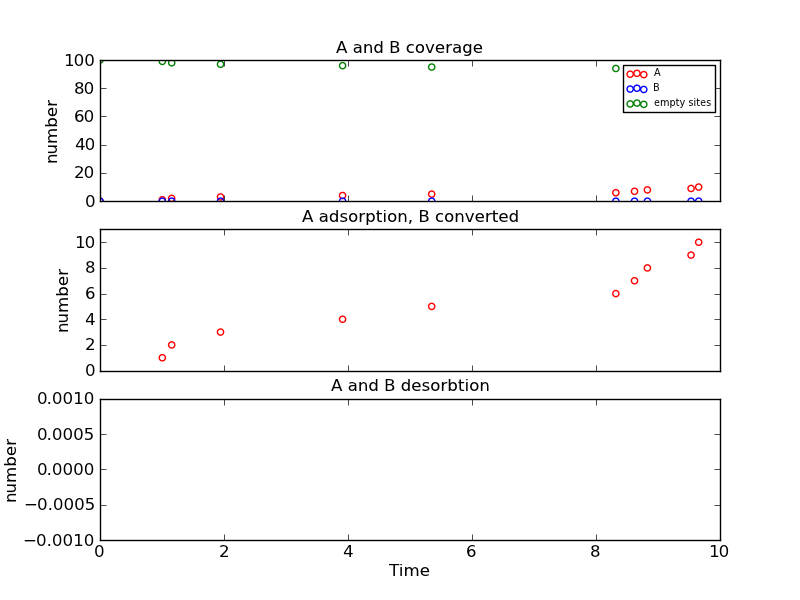
\includegraphics[width=3.5in, height=4.2in]{./coadsorb_irreversible/AtoBirreversible10x10_101_Ades2x_EAx10E3_EB5E3_3.png} &
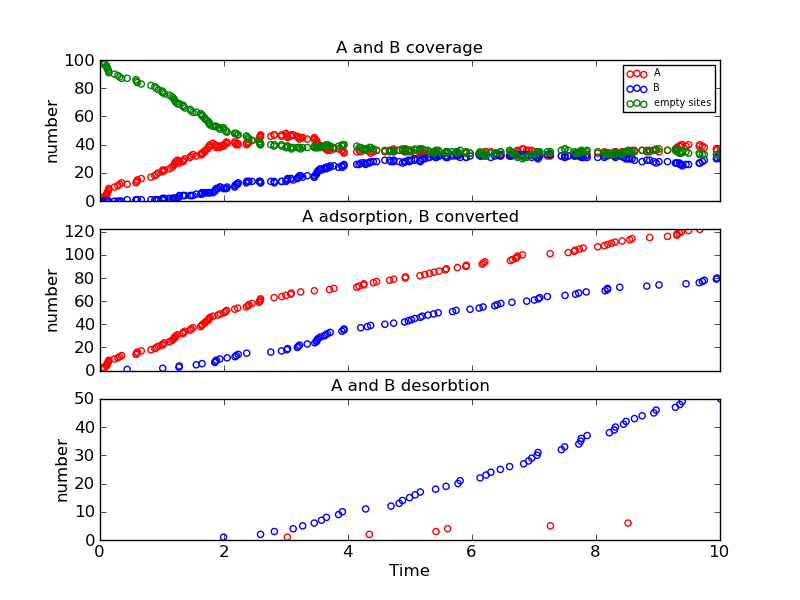
\includegraphics[width=3.5in, height=4.2in]{./coadsorb_irreversible/AtoBirreversible10x10_201_Ades2x_EAx10E3_EB5E3_3.png} \\
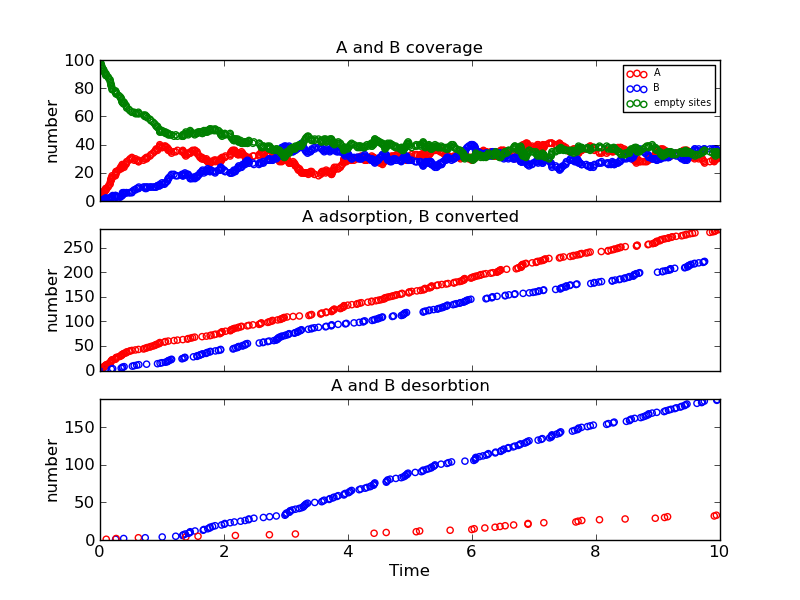
\includegraphics[width=3.5in, height=4.2in]{./coadsorb_irreversible/AtoBirreversible10x10_301_Ades2x_EAx10E3_EB5E3_3.png} &
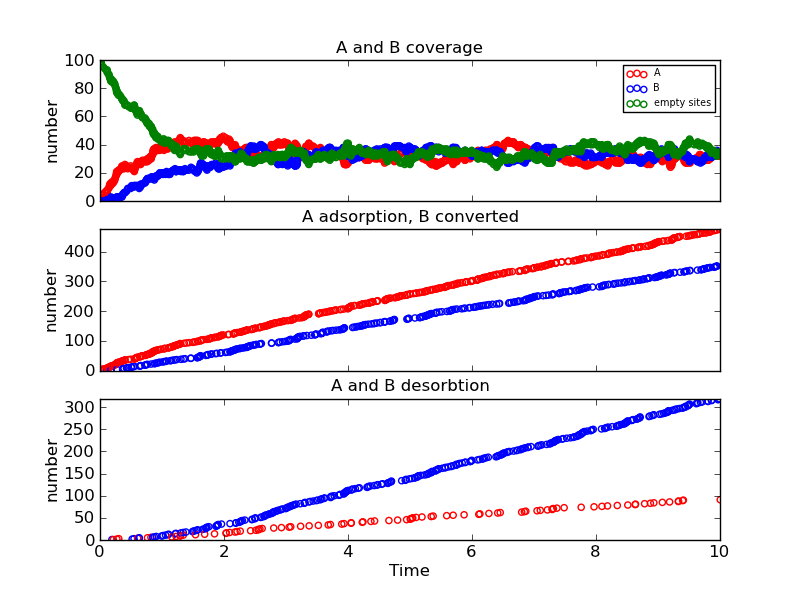
\includegraphics[width=3.5in, height=4.2in]{./coadsorb_irreversible/AtoBirreversible10x10_401_Ades2x_EAx10E3_EB5E3_3.png} 
\end{tabular}
\caption{This figure describes the (top of three:) total coverage of the systems simulated, (middle of three:) absorption of the particles present, (bottom of three:) and desorption of the particles present on a 10x10 lattice, where the transition coefficients to not depend on the position of the lattice. In these simulations, the activation energy of desorption of A is twice as large as any other event , where the activation energy is E$_{a_{A:desorption}}$=10kJmol$^{-1}$ and E$_{a_{other}}$=5kJmol$^{-1}$. [From top left to bottom right:] 101 K, 201 K, 301 K, 401 K. }
\end{figure}

\setlength{\unitlength}{1in}
\begin{figure}[h!]
\begin{tabular}{cc}
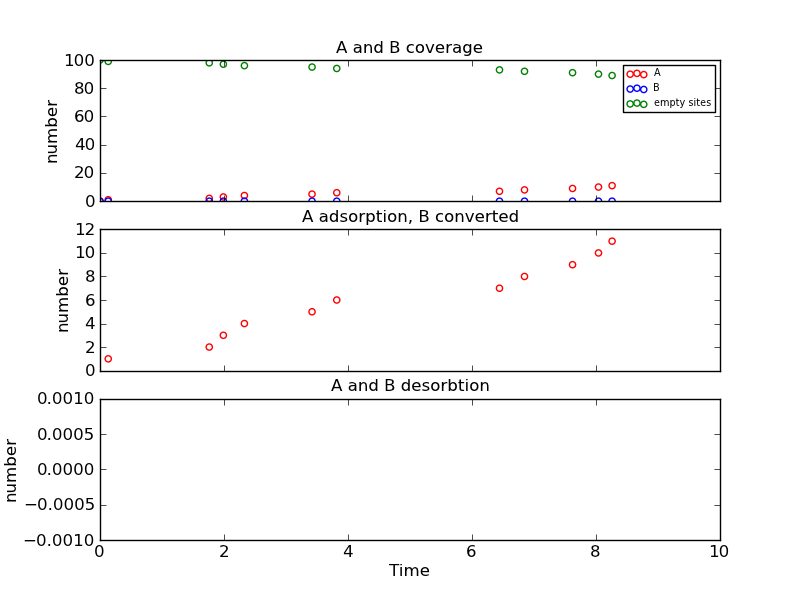
\includegraphics[width=3.5in, height=4.2in]{./coadsorb_irreversible/AtoBirreversible10x10_101_Bdes2x_EA5E3_EBx10E3_3.png} &
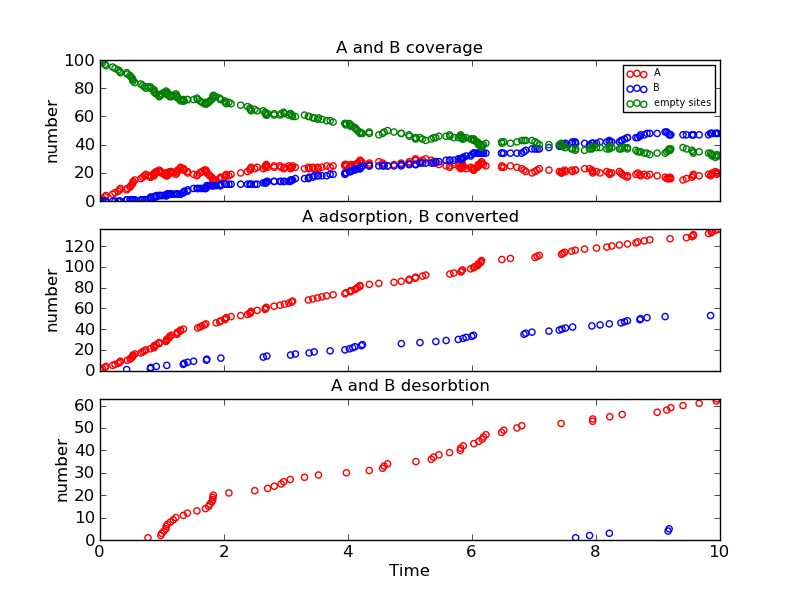
\includegraphics[width=3.5in, height=4.2in]{./coadsorb_irreversible/AtoBirreversible10x10_201_Bdes2x_EA5E3_EBx10E3_3.png} \\
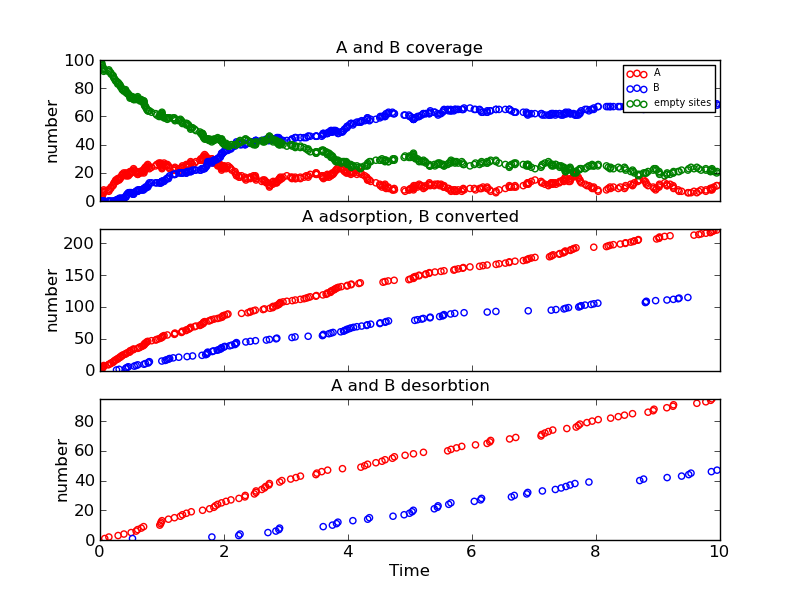
\includegraphics[width=3.5in, height=4.2in]{./coadsorb_irreversible/AtoBirreversible10x10_301_Bdes2x_EA5E3_EBx10E3_3.png} &
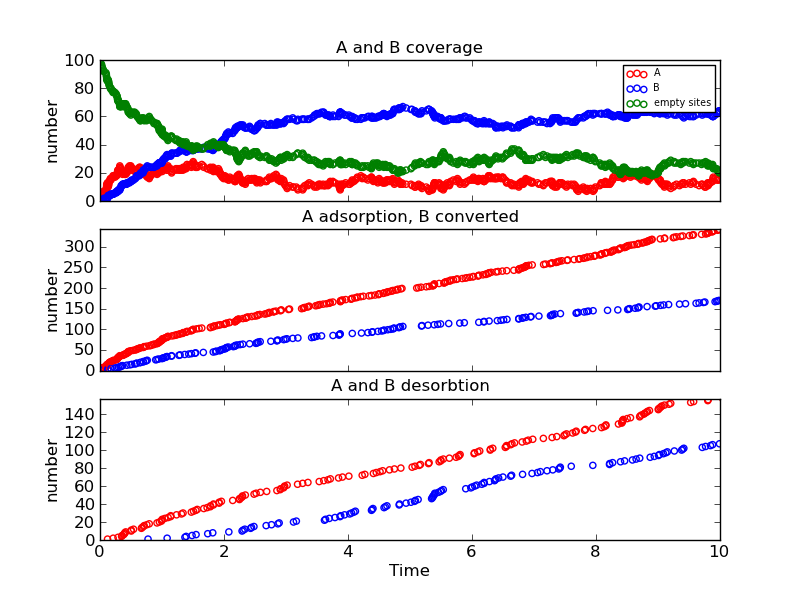
\includegraphics[width=3.5in, height=4.2in]{./coadsorb_irreversible/AtoBirreversible10x10_401_Bdes2x_EA5E3_EBx10E3_3.png} 
\end{tabular}
\caption{This figure describes the (top of three:) total coverage of the systems simulated, (middle of three:) absorption of the particles present, (bottom of three:) and desorption of the particles present on a10x10 lattice, where the transition coefficients to not depend on the position of the lattice. In these simulations, the activation energy of desorption of B is twice as large as that of any other event, where the activation energy is E$_{a_{B:desorption}}$=10kJmol$^{-1}$ and E$_{a_{other}}$=5kJmol$^{-1}$. [From top left to bottom right:] 101 K, 201 K, 301 K, 401 K.}
\end{figure}

\setlength{\unitlength}{1in}
\begin{figure}[h!]
\begin{tabular}{cc}
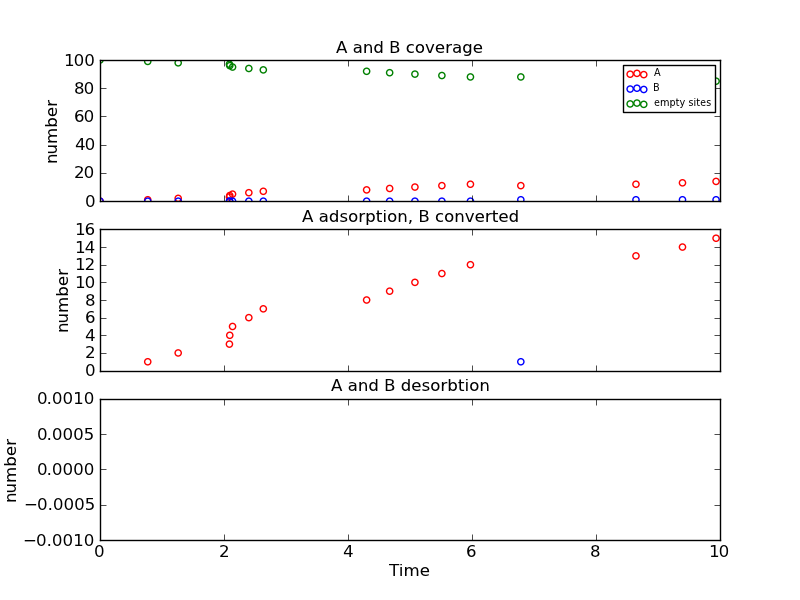
\includegraphics[width=3.5in, height=4.2in]{./coadsorb_irreversible/AtoBirreversible10x10_101_desorb2x_Ea5E3_Ed10E3_3.png} &
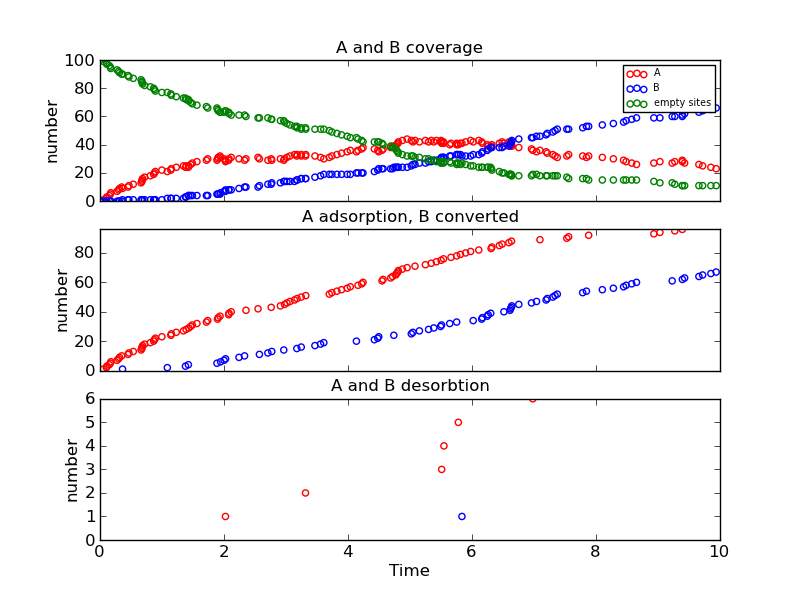
\includegraphics[width=3.5in, height=4.2in]{./coadsorb_irreversible/AtoBirreversible10x10_201_desorb2x_Ea5E3_Ed10E3_3.png} \\
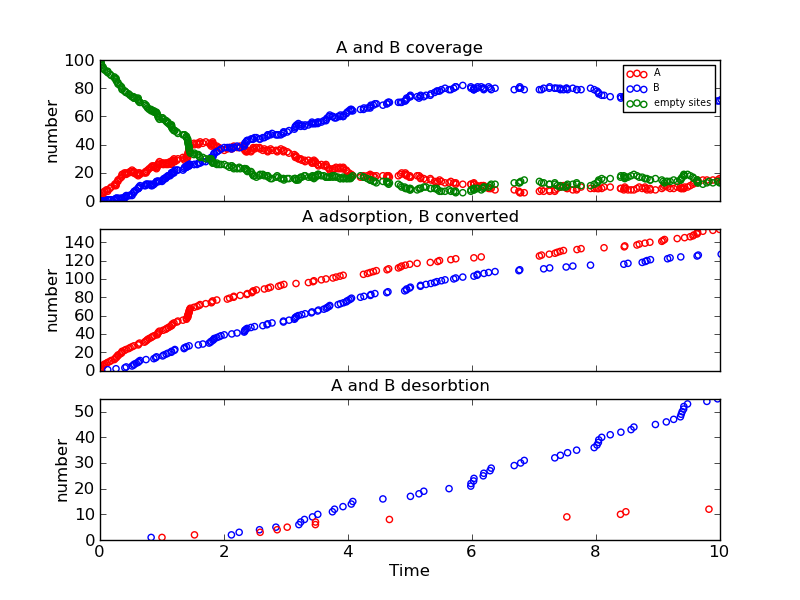
\includegraphics[width=3.5in, height=4.2in]{./coadsorb_irreversible/AtoBirreversible10x10_301_desorb2x_Ea5E3_Ed10E3_3.png} &
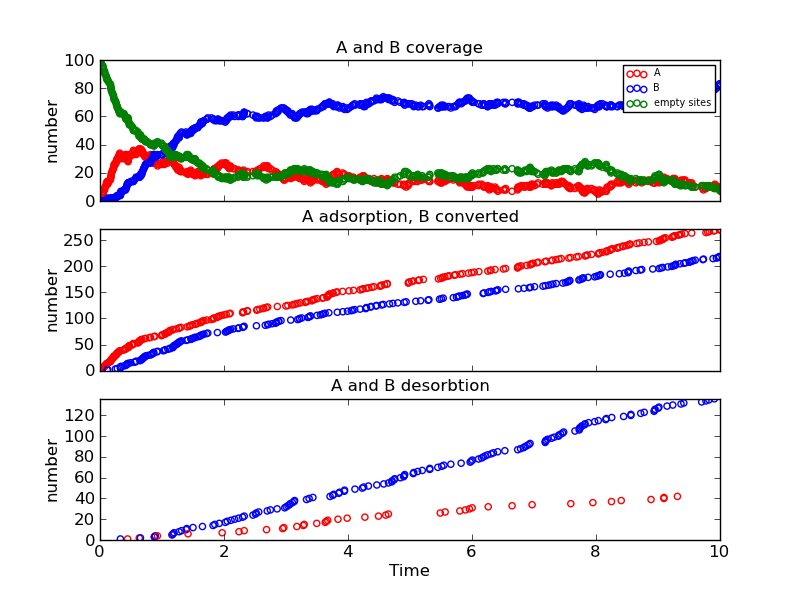
\includegraphics[width=3.5in, height=4.2in]{./coadsorb_irreversible/AtoBirreversible10x10_401_desorb2x_Ea5E3_Ed10E3_3.png}
\end{tabular}
\caption{This figure describes the (top of three:) total coverage of the systems simulated, (middle of three:) absorption of the particles present, (bottom of three:) and desorption of the particles present on a 10x10 lattice, where the transition coefficients to not depend on the position of the lattice. In these simulations, the activation energy of desorption of A and B is twice as large as that of any other event, where the activation energy is E$_{a_{desorption}}$=10kJmol$^{-1}$ and E$_{a_{absorption}}$=5kJmol$^{-1}$. [From top left to bottom right:] 101 K, 201 K, 301 K, 401 K. }
\end{figure}

\setlength{\unitlength}{1in}
\begin{figure}[h!]
\begin{tabular}{cc}
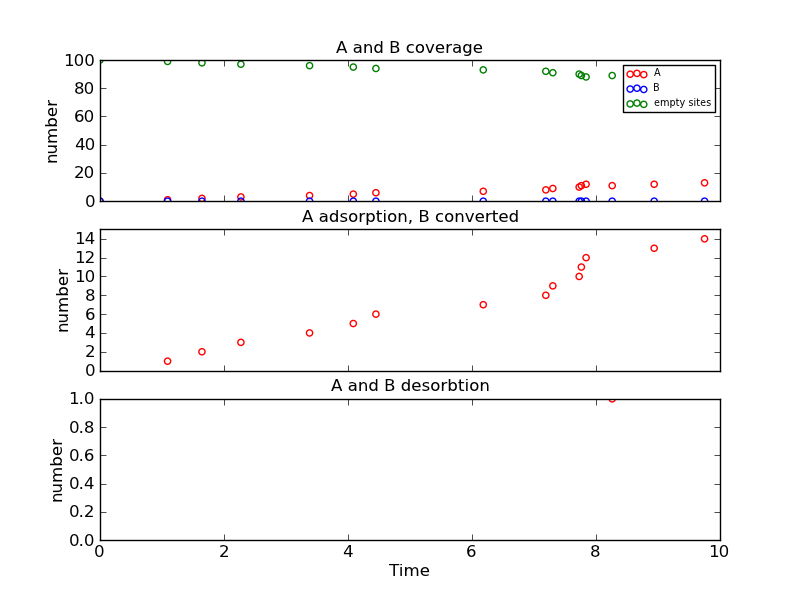
\includegraphics[width=3.5in, height=4.2in]{./coadsorb_irreversible/AtoBirreversible10x10_101_AtoB2x_Ea5E3_Eirr10E3_3.png} &
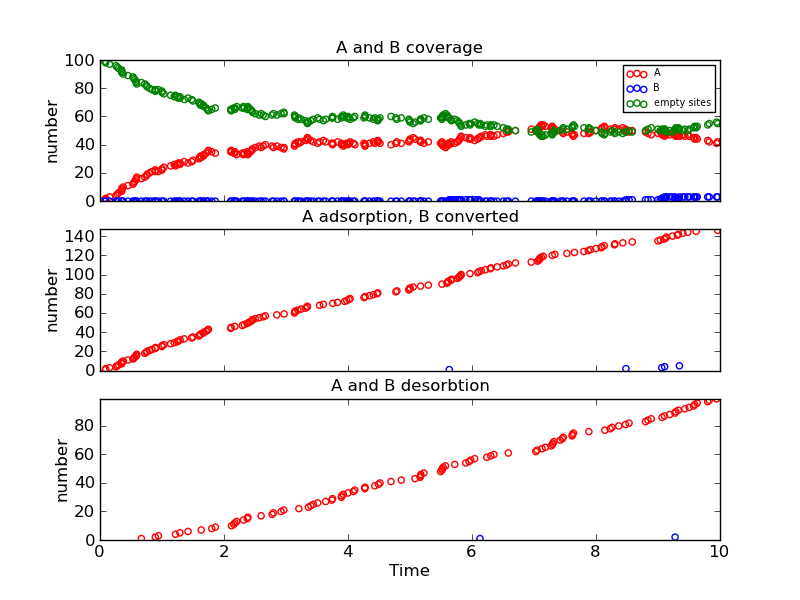
\includegraphics[width=3.5in, height=4.2in]{./coadsorb_irreversible/AtoBirreversible10x10_201_AtoB2x_Ea5E3_Eirr10E3_3.png} \\
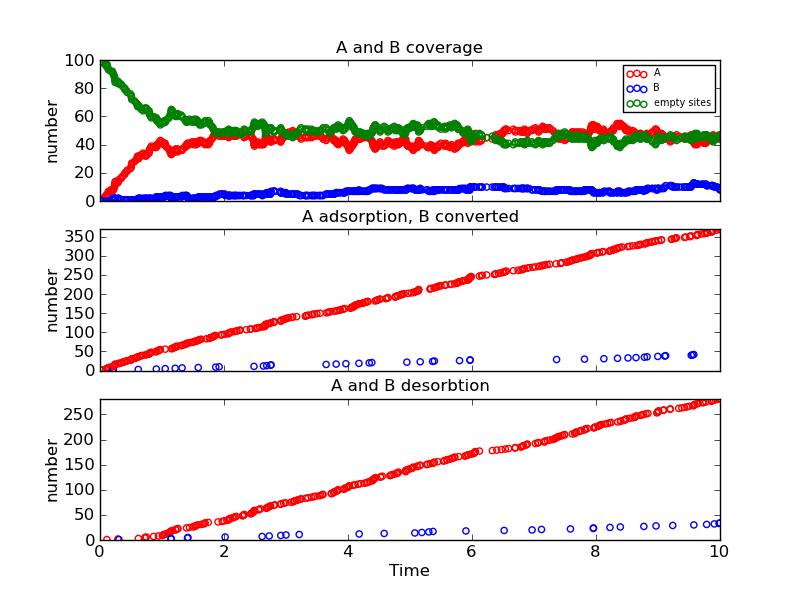
\includegraphics[width=3.5in, height=4.2in]{./coadsorb_irreversible/AtoBirreversible10x10_301_AtoB2x_Ea5E3_Eirr10E3_3.png} &
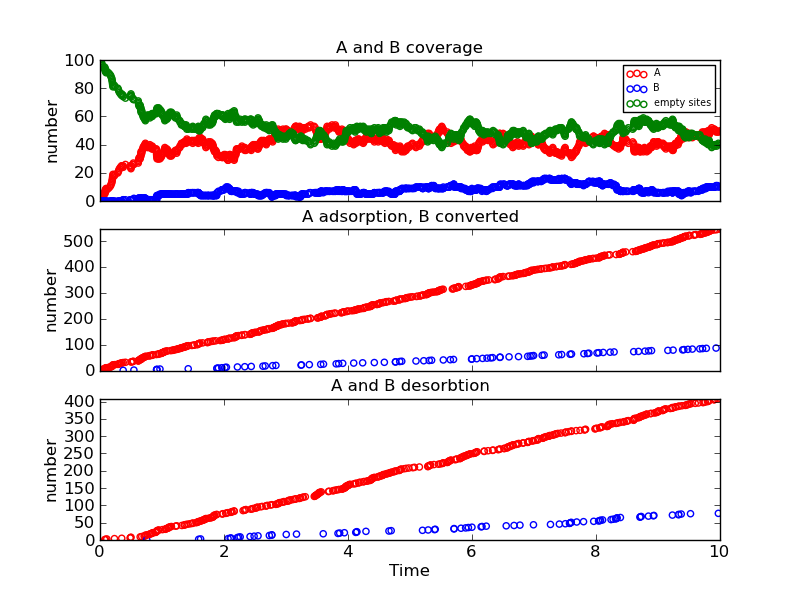
\includegraphics[width=3.5in, height=4.2in]{./coadsorb_irreversible/AtoBirreversible10x10_401_AtoB2x_Ea5E3_Eirr10E3_3.png}
\end{tabular}
\caption{This figure describes the (top of three:) total coverage of the systems simulated, (middle of three:) absorption of the particles present, (bottom of three:) and desorption of the particles present on a 10x10 lattice, where the transition coefficients to not depend on the position of the lattice. In these simulations, the activation energy associated with catalytic conversion of A to B is twice as large as that of all other events, where the activation energy is E$_{a_{A:B}}$=10kJmol$^{-1}$ and E$_{a_{other}}$=5kJmol$^{-1}$. [From top left to bottom right:] 101 K, 201 K, 301 K, 401 K. }
\end{figure}



\end{document}